% oil_mc_pres.tex
%Last updated April 1st, 2015

\documentclass{beamer}
\usepackage{url} 
\usepackage{amsmath}
\usepackage{esdiff} %for writing partial derivatives

\usetheme{default}

\title{Estimating the Effect of Price on Oil Field Production: Evidence from the Norwegian Continental Shelf}
\author{Johannes Mauritzen}
\institute % (optional)
{
 Department of Business and Management Science\\
 NHH Norwegian School of Economics
}
%\logo{\includegraphics[height=1.5cm]{/Users/johannesmauritzen/Google Drive/Logos/NHH.jpg}}

\date{April 2, 2015}


\begin{document}

%--- the titlepage frame -------------------------%
\begin{frame}[plain]
  \titlepage
\end{frame}

\begin{frame}
	\begin{figure}
		\includegraphics[width=1\textwidth]{figures/oil_decline_print.png}
		% \caption{The production profile for the entire Norwegian Continental Shelf is bell-shaped, reflecting the correlated production profiles of the fields.  With oil prices that are autocorrelated, }
		\label{oil_decline}
	\end{figure}
\end{frame}

\begin{frame}[plain]
	\begin{itemize}
		\item Effect of Price on Drilling / Reserve Replacement
			\begin{itemize} \item Mohn and Osmundsen (2008), Mohn (2008), Ringlund (2008) \end{itemize}
		 \item Aggregate Production

			\begin{itemize}
				\item Curve-fitting/Simulation (geo-engineering)
				\item Econometric
			
				\begin{itemize}
					\item Kaufman (1990), Kaufman and Cleveland (2001)
					\item Ramcharran (2002)
	 			\end{itemize}		
	 	\end{itemize}
	 	\item Field-level
	 			\begin{itemize}
	 				\item Rao (2012)
	 			\end{itemize}
	\end{itemize}
\end{frame}

\begin{frame}[plain]
	Generalized Additive Models
	\begin{itemize}
	\item  Hastie and Tibshirani (1990) 
	\item  Wood (2006)
	\end {itemize}
\end{frame}

\begin{frame}[plain]
	Main Results
	\begin{itemize}
		\item No significant contemporary effect of oil price on field production (within 3 years)
		\item Slight lagged effect found after 4-8 years, magnitude of around 2\%
		\item Most of this effect seems to come in the planning stage of an oil field
		\item Little to no effect - contemporary or lagged - in depleting fields
	\end{itemize}
\end{frame}

\begin{frame}[plain]
	\begin{figure}
	\includegraphics[width=.8\textwidth]{figures/north_sea_reserves.png}	
	\label{north_sea_reserves}
	\end{figure}
\end{frame}

\begin{frame}[plain]
	\begin{figure}
	\includegraphics[width=.8\textwidth]{figures/norwegian_sea_reserves.png}
	
	\label{norwegian_sea_reserves}
	\end{figure}
\end{frame}

\begin{frame}[plain]

\begin{figure}
	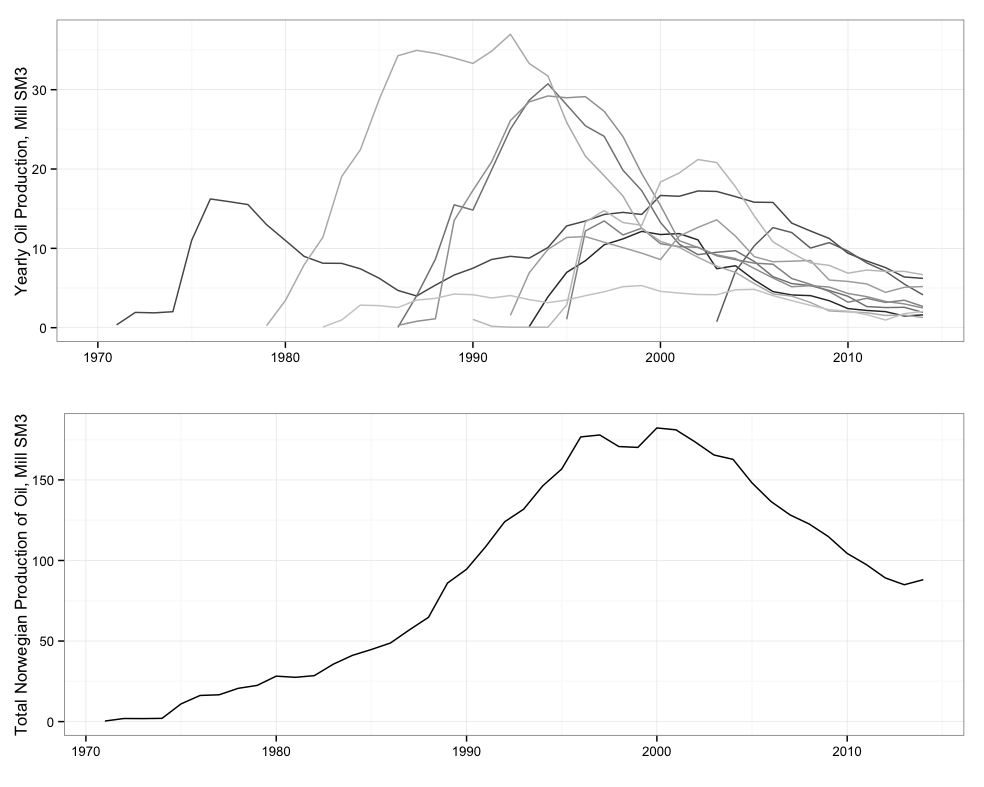
\includegraphics[width=.8\textwidth]{figures/oil_decline.png}
	
	\label{oil_decline}
\end{figure}

\end{frame}


\begin{frame}[plain]
	\begin{figure}
	\includegraphics[width=.8\textwidth]{figures/top10_production.png}
	
	\label{top10_production}	
	\end{figure}
\end{frame}

\begin{frame}
	\begin{figure}
		\includegraphics[width=1\textwidth]{figures/statfjord_dem_print.png}
		\label{statfjord_dem}
	\end{figure}
\end{frame}

\begin{frame}[plain]
	\begin{equation}
		\begin{split}
		 Log(Production_{i,t}) & = \alpha_0 + Poly(time\_to\_peak_{i,t}) \\ 
		 & +  Poly(peak\_to\_end_{i,t}) \\
		 & + \gamma total\_recoverable\_oil_i \\
		 & + \beta oil\_price_{t,t-1, t-2,.., t-n} + \epsilon
		\end{split}
	\label{glm_eqn}
	\end{equation}
\end{frame}

\begin{frame}[plain]
	\begin{figure}
		\includegraphics[width=.8\textwidth]{figures/glm_dirty_box.png}
		\label{glm_dirty_box}
	\end{figure}
\end{frame}



\begin{frame}[plain]
	\begin{equation}
	\begin{split}
		Log(Production_{i,t})&=f(time\_to\_peak_{i,t}, total\_recoverable\_oil_i) \\
		& \quad + f(peak\_to\_end_{i,t}, total\_recoverable\_oil_i) \\
		& \quad + \beta oil\_price_{t,t-1, t-2,.., t-n} + \epsilon
	\end{split}
	\label{gam_price_eqn}
	\end{equation}
\end{frame}

\begin{frame}[plain]
	\begin{equation}
	Production_{t}=f(time) + \epsilon
		\label{simp_eqn}
	\end{equation}
\end{frame}


\begin{frame}[plain]
	\begin{figure}
		\includegraphics[width=.8\textwidth]{figures/statfjord_gam.png}
		
		\label{statfjord_gam}
	\end{figure}
\end{frame}


\begin{frame}[plain]
	\begin{equation}
	\begin{split}
		Log(Production_{i,t})&=f(time\_to\_peak_{i,t}, total\_recoverable\_oil_i) \\
		& \quad + f(peak\_to\_end_{i,t}, total\_recoverable\_oil_i) \\
		& \quad + \beta oil\_price_{t,t-1, t-2,.., t-n} + \epsilon
	\end{split}
	\label{gam_price_eqn}
	\end{equation}
\end{frame}


\begin{frame}[plain]
	Thin Plate (Regression) Splines (Duchon 1977)
	\begin{equation}
	y_i = g(x_1, x_2)
	\end{equation}

	\begin{equation}
	\min \|\boldsymbol{y-f}\|^2 + \lambda J_{md}(f)
	\end{equation}

	\begin{equation}
	J_{22}{f}= \diffp[2]{f}{x_1}^2 + \diffp[2]{f}{{x_1}{x_2}} + \diffp[2]{f}{x_2}^2dx_1 dx_2
	\end{equation}
\end{frame}

\begin{frame}[plain]	
	\begin{figure}
	Build-out Phase
	\includegraphics[width=1\textwidth]{figures/gam_prepeak_pres.png}
	% \caption{The estimated coefficients on the price terms in a model of fields in the build-out phase.  For large fields, positive coefficients are estimated at the 6th, 7th and 8th lag, but the estimates are imprecise and not statistically significant.  Significant positive coefficients are estimated for small fields at the fifth and eighth lag.  In a pooled model, significant positive coefficients are found at the fourth through eight lags.}
	\label{gam_prepeak_print}
	\end{figure}
\end{frame}

\begin{frame}[plain]
	\begin{figure}
	Depletion Phase
	\includegraphics[width=1\textwidth]{figures/gam_postpeak_print.png}
	% \caption{The estimated coefficients on the price terms in a model of oil field production in depleting fields.  No significant coefficients are estimated except for on the 8th lag of small fields.  This effect is not, however, robust to changes in specification.}
	\label{gam_postpeak_pres}
	\end{figure}
\end{frame}

\begin{frame}[plain]
	\begin{figure}
		\includegraphics[width=.8\textwidth]{figures/field_time_to_peak_pres.png}		
		\label{field_time_to_peak}
	\end{figure}
\end{frame}



\begin{frame}
\begin{figure}
	\includegraphics[width=1\textwidth]{figures/oil_price_series.png}
	\label{oil_price_series}	
\end{figure}
\end{frame}


\begin{frame}[plain, fragile]
Monte-Carlo Simulation Sudo-code
	\begin{verbatim}
	>Generate X fields with size
	 from exponential-normal distribution
	>Generate random starting year for each field
	>Generate logistic cumulative production profile
	\end{verbatim}
\end{frame}

\begin{frame}[plain, fragile]
	\begin{verbatim}
		In loop:
			>Create production profiles from derivative of
			logistic function, price component
			 and stochastic component
			>Regress ``fake'' data with GLM and GAM model
			>Store point estimates
	\end{verbatim}
\end{frame}

\begin{frame}
	\begin{equation}
		\begin{split}
		cumProd&=\frac{size}{1+exp(\frac{-prodTime_t}{3})} \\
		log(production) &= f`(time) + beta*log(price) + epsilon
		\end{split}
	\end{equation}
\end{frame}

\begin{frame}[plain, fragile]
	\begin{equation}
		\begin{split}
		prod_t&=poly(prod\_time_t) + field\_size_i \\
		prod_t&=s(prod\_time,field\_size_i) + \beta price_t
		\end{split}
	\end{equation}
\end{frame}

\begin{frame}[plain]
	\begin{figure}
		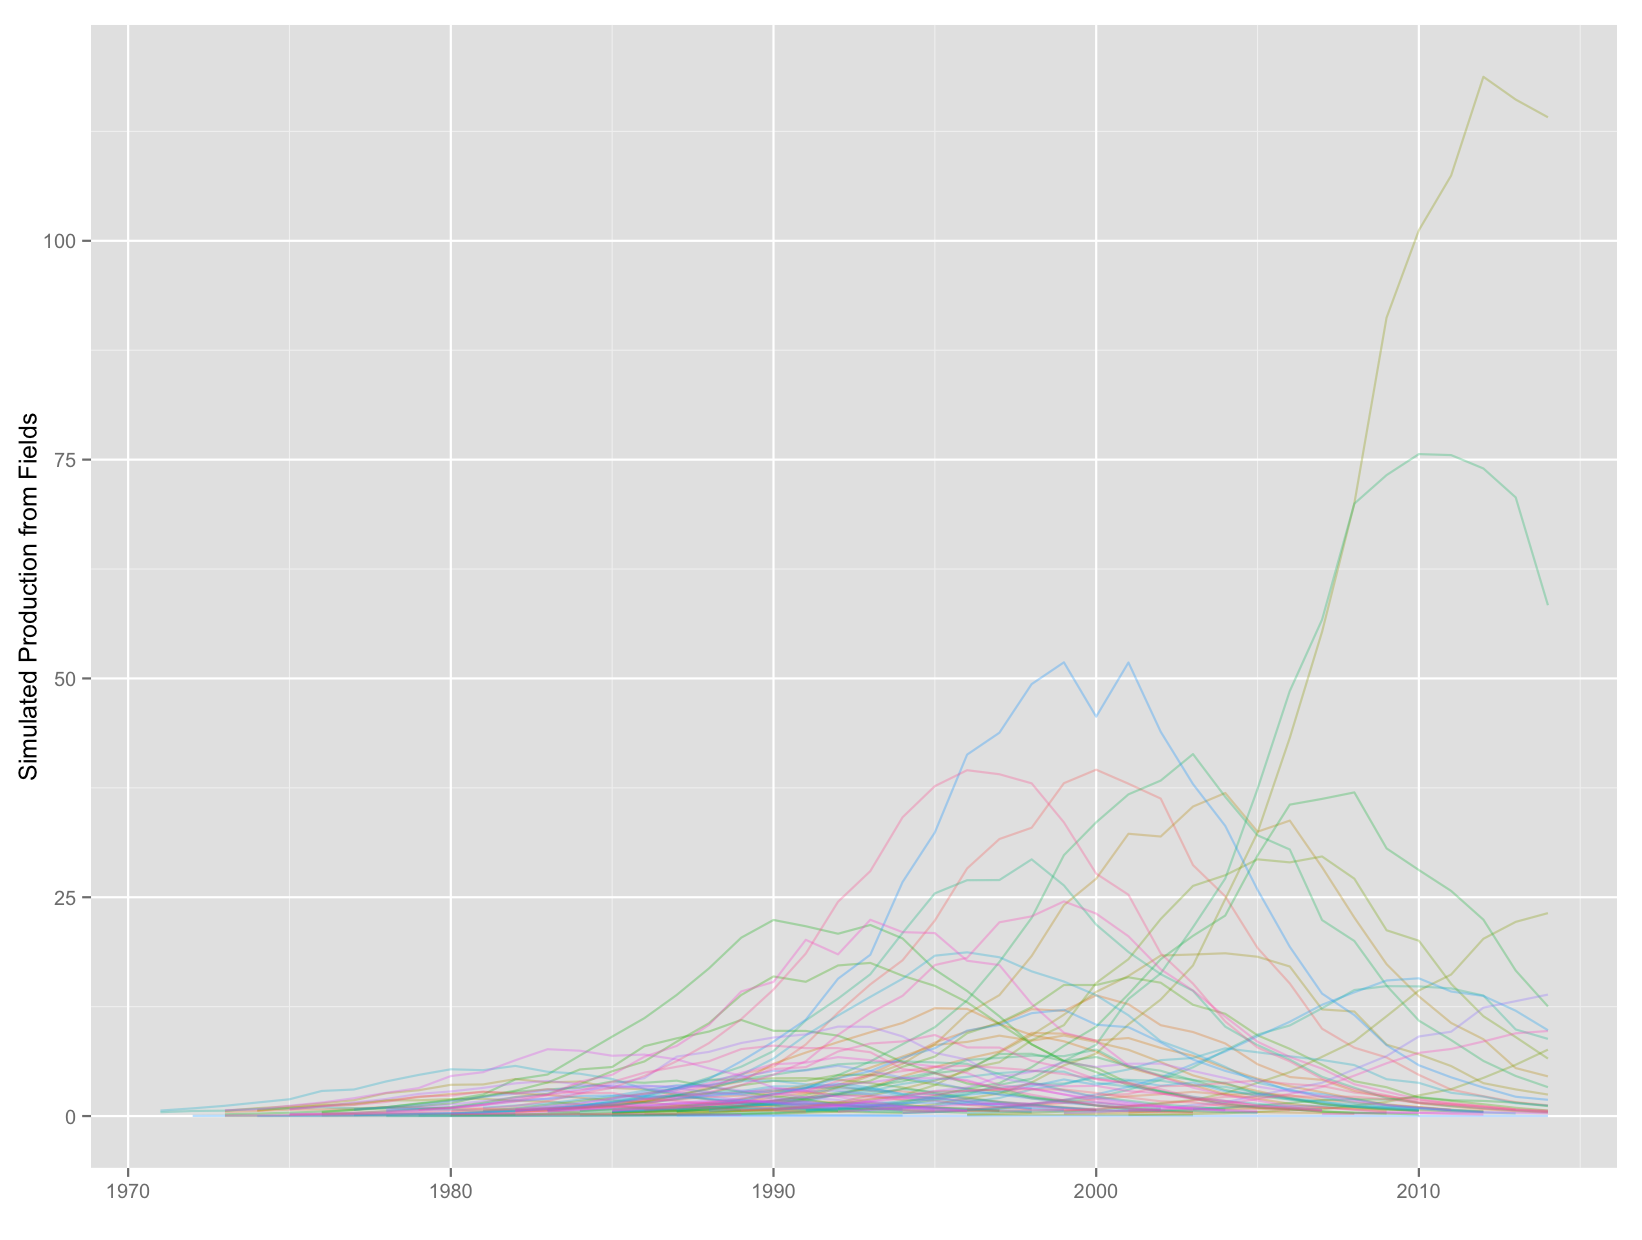
\includegraphics[width=1\textwidth]{figures/simulated_production.png}
		\caption{Simulated production of 77 oil fields}
		\label{simulated_production}	
	\end{figure}
\end{frame}

\begin{frame}[plain]
	\begin{figure}
		\includegraphics[width=1\textwidth]{figures/lin_model_price_mc.png}
		\caption{Estimated coefficients on price from linear model from Monte Carlo Experiment}
		\label{lin_model_price_mc}	
	\end{figure}
\end{frame}

\begin{frame}[plain]
	\begin{figure}
		\includegraphics[width=1\textwidth]{figures/gam_model_price_mc.png}
		\caption{Estimated coefficients on price from GAM model from Monte Carlo Experiment}
		\label{gam_model_price_mc.png}	
	\end{figure}
\end{frame}




\begin{frame}[plain]
	\begin{figure}
		\includegraphics[width=.8\textwidth]{figures/tot_forecast.png}
		
		\label{tot_forecast}
	\end{figure}
\end{frame}


\begin{frame}[plain]
\begin{figure}
		\includegraphics[width=.8\textwidth]{figures/NPD_oil_forecast.png}
		
		\label{NPD_oil_forecast}
	\end{figure}
\end{frame}

\begin{frame}[plain]
	\begin{itemize}
	\item[] Criticisms
		\begin{itemize}
			\item Ignores significant technical changes in the oil industry
		\end{itemize}
	\end{itemize}
\end{frame}

\begin{frame}[plain]
	\begin{itemize}
	\item[] Criticisms
		\begin{itemize}
			\item Ignores significant technical changes in the oil industry
			\item Estimate of field size itself is affected by price
		\end{itemize}
	\end{itemize}
\end{frame}

\begin{frame}[plain]
	\begin{itemize}
	\item[] Criticisms
		\begin{itemize}
			\item Ignores significant technical changes in the oil industry
			\item Field size itself is affected by price
			\item Time at which production peaks, as measured from the start of production, is likely affected by price as well
		\end{itemize}
	\end{itemize}
\end{frame}

\begin{frame}[plain]
	\begin{itemize}
	\item[] Criticisms
		\begin{itemize}
			\item Ignores significant technical changes in the oil industry
			\item Field size itself is affected by price
			\item Time at which production peaks, as measured from the start of production, is likely affected by price as well
			\item Costs in industry are correlated with oil price
		\end{itemize}
	\end{itemize}
\end{frame}

\begin{frame}
	\begin{itemize}
		\item[] johannes.mauritzen@nhh.no 
		\item[] jmaurit.github.io\#oil\_prices
	\end{itemize}
\end{frame}

\end{document}